\section{State Space Analysis}
\label{sec:State_Space_Analysis}

\subsection{Experimental Deployment}

Consider the sample deployment shown in Figure \ref{fig:CT}. This is a 3-satellite cluster with each satellite consisting of an instance of a DREMS application. All satellites are deployed with the same component assembly and Satellite 1 is chosen as the cluster leader using a leader-election algorithm. 

\begin{figure}[htb]
	\centering
	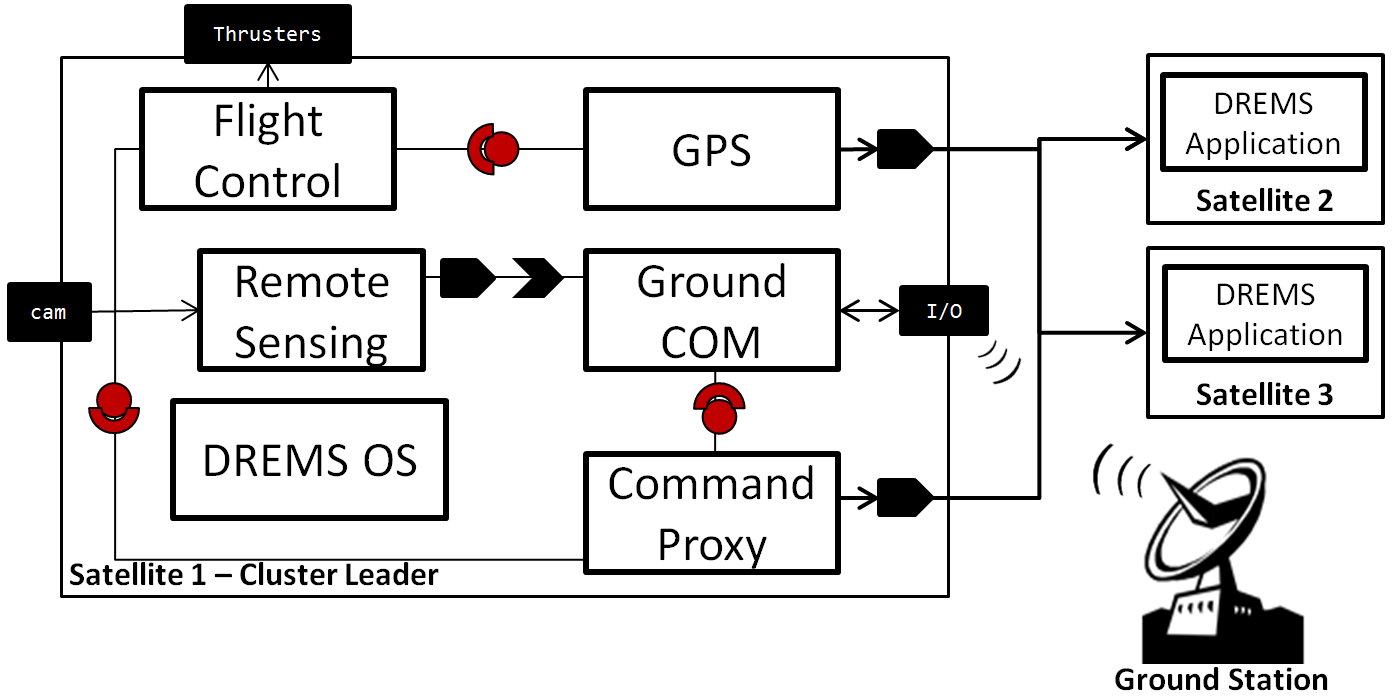
\includegraphics[width=0.48\textwidth]{figs/Case_Study_Fixed.png}
	\caption{DREMS Application}
	\label{fig:CT}
\end{figure}

Each satellite consists of a set of sensor-dependent critical components required for both safe flight and remote sensing tasks. These components interact with physical sensor devices such as cameras, radar altimeters etc. to receive and process data periodically and transmit to a ground receiving station. The component \emph{Ground COM} behaves as the communication link between internal satellite components and the ground station. Periodically processed and encoded image data from the \emph{Remote Sensing} device is received by the Ground COM using a DDS-based \emph{publish-subscribe} scheme upon which the data is transmitted to the ground receiver. 

A more critical task in this deployment is maintaining the cluster attitude. This includes the relative position and acceleration of the satellites from each other with the satellites using a distributed but synchronized database to keep track of \emph{state vectors} of each other. A \emph{GPS} component periodically publishes a state vector to all satellites in the cluster. The GPS component uses its subscriber port to receive the equivalent vectors from other satellites. A \emph{Flight Control} component responsible for the integrity of the cluster flight uses an RMI interface to access the most recent vector metrics from GPS including metrics received from other satellites to calculate and maintain the flight trajectory. The Flight Control component does not fetch GPS information until all the satellites have published on the updated sensor data. 

Lastly, there are scenarios where the ground station will command the satellites in the cluster to perform a coordinated \emph{scatter}. This is a time-triggered critical event that is transmitted to the cluster leader. On receiving such a command, the Ground COM of Satellite 1 uses an interface on the \emph{Command Proxy} to publish this command to all satellites in the cluster. The command proxy uses a high-priority synchronous method invocation to communicate with the Flight Control component to trigger the scatter. Since the component-level scheduler is non-preemptive, the Flight Control cannot trash any operation that it would be executing at time $t_S$ when a scatter request is received from the Command Proxy. This motivates the need for accurate modeling of component interaction semantics to obtain conservative response-time results. 

\begin{figure}[htb]
	\centering
	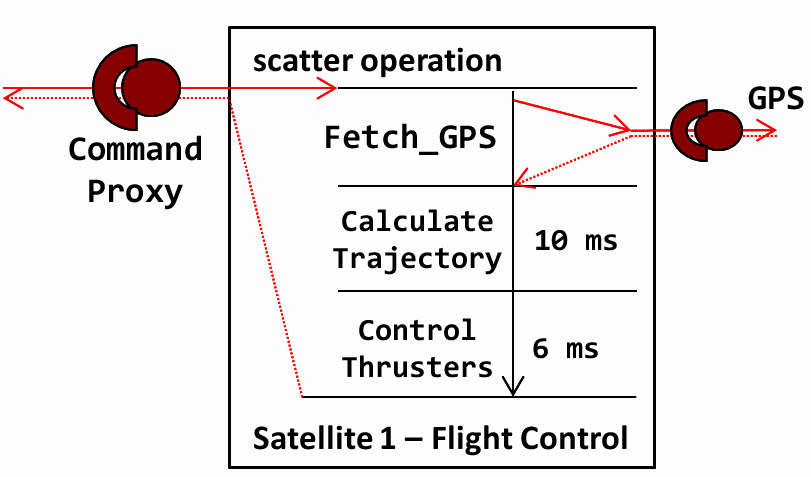
\includegraphics[width=0.45\textwidth]{figs/scatter.jpg}
	\caption{Scatter Operation}
	\label{fig:FLC}
\end{figure}

The abstract business logic \emph{steps} of the \emph{scatter} operation in the Flight Control is modeled as shown in Figure \ref{fig:FLC}. This operation is requested by the Command Proxy when a command is received from the ground station. For sake of simplicity, we have reduced this operation down to 3 distinct steps. The controller first obtains updated position vectors from the GPS component using the RMI interface. Notice the lack of a WCET for this interaction. This is because the GPS is scheduled on a separate temporal partition and the amount of time for which the Flight Control has to wait for the updated metrics is dependent on the time stamp at which the scatter command is received and also the state of the GPS component message queue. Once these metrics are received, the Flight Control calculates a new trajectory which is also the return arguments of this operation. This trajectory is passed down to the Command Proxy which publishes the leader's updated metrics to the rest of the satellites in the cluster. Once the trajectory is calculated, each Flight Control component interacts with the thrusters and maneuvers the satellites.  

\subsubsection{Temporal Partitioning}

The temporal partitioning schedule for this scenario consists of two broad minor frames each of length 100 msec. All satellite sensor components such as the camera and the GPS are grouped into sensor processes and assigned to the first temporal partition. This includes the image processing tasks undertaken by the Remote Sensing component, the vector publication and reception by the GPS component and the communication with the ground network. 

The Flight Control is assigned to partition 2 and is guaranteed to receive the newest vector data as it waits for the GPS component to update the database of state variables. The Ground COM and the Command Proxy component threads run at SYSTEM priority and are scheduled as and when required. In our case, we use a sporadic timer on the Ground COM component to trigger the sequence of interactions leading a scatter.


\subsection{State Space Exploration}


The CPN Tools uses a built-in state space (SS) analysis tool to generate a bounded state space from an initialized CPN model. Exceptions caused by inconsistent token structures or incomplete arc bindings cause the tool to stop generation. However, it has been noted by the CPN Tools community that the built-in state space tool is inefficient with its search algorithm \cite{CPNTwoInterfaces} and therefore we also work with the ASAP tool \cite{ASAP} which is an extensible platform for advanced CPN state space analysis methods including optimized reduction techniques for large-scale applications. Thirdly, we also use the ASK-CTL \cite{ASK-CTL} model checking library, expressing state space properties using a CTL-style logic and exploiting strongly connected components for efficient state space searching. For smaller design models, we use observer places \cite{Alpern1989} in the CPN to \emph{collect} tokens that represent timing anomalies such as deadline violations. This makes the state space search easier as we simply look for nodes where the observer places are not empty. 

\subsubsection{Bounded State Space Generation}

Components in safety-critical DRE applications can be either sporadically or periodically triggered by an entity. A bounded state space generated in CPN Tools must be sufficiently large so that the lack of deadline violations or deadlocks or delayed response times \emph{during} this interval will guarantee safe operation throughout the lifetime of the components. This is important in order to gain confidence from the obtained results while not generating an infinite state space. 

\subsubsection{Deadline Violations and System-wide Deadlocks}

On a sufficiently large bounded state space, the analysis tool looks for specific behavioral patterns such as weakly-decreasing size of the component message queue. If requests from external components or timers pile up over time in the message queue, the responsible component is not scheduled for long enough time to be able to serve all the requests on time. This observation will also be supported by the detection of deadline violations or unusual blocking times. This is especially useful in identifying timing delays that propagate through successive hyperperiods in the temporal partition schedule. 

\begin{figure}[htb]
	\centering
	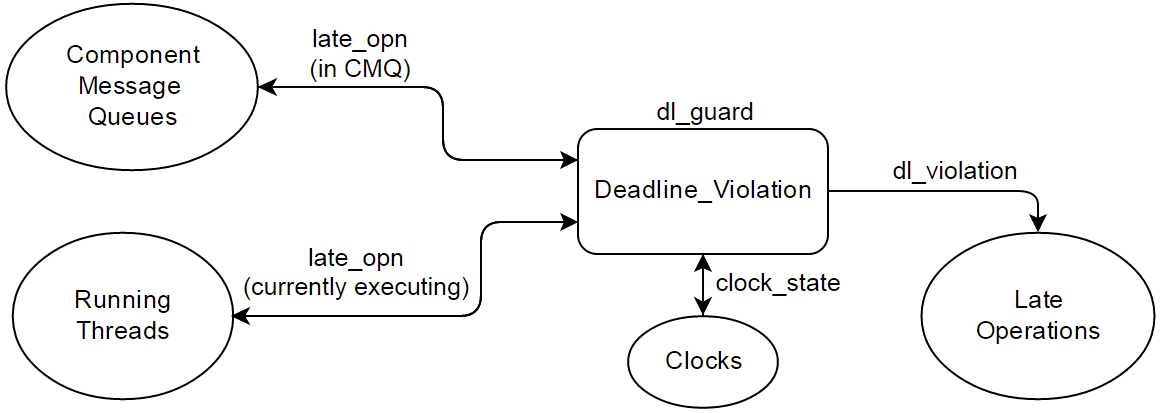
\includegraphics[width=0.48\textwidth]{figs/Deadline_Violations.png}
	\caption{Deadline Violation Observer place}
	\label{fig:DL}
\end{figure}

As mentioned earlier, our model uses an observer place for deadline violation detection, especially in small/medium sized applications. A \emph{Deadline\_Violation} (Figure \ref{fig:DL}) transition fires at any point in time when the guard \emph{dl\_guard} is satisfied and arc bindings are realized with its input places. The transition observes the states of the currently running threads and the component message queues to identify deadline violations on operations that are either executing or waiting to execute. The \emph{dl\_violation} tokens in \emph{Late Operations} ($LO$) is of the form:

\vspace{-0.1in}
\begin{equation}
\label{eq:DLV}
LO = \ <Node_{name}, O_{name}, O_{ST}, \ O_{DLT}>
\end{equation}

where operation $O_{name}$ executing on computing node $Node_{name}$ started at time $O_{ST}$ and violated its deadline at time $O_{DLT}$. Since the component-level scheduler uses a non-preemptive scheme, this operation is still run to completion after the violated deadline. Delays like these propagate to the waiting operations in the message queue.

\begin{table*}[t]
	\caption{Component Operations on Satellite 1}
	\label{table:AR}
	\begin{center}
		\begin{tabular}{ | c | p{2.0cm} | p{1.7cm} | p{1.7cm} | p{1.7cm} | p{1.9cm} | p{1.9cm} |}
			\hline
			Component & \multicolumn{1}{|c|}{Operation} & $Dl_{O}$ (ms) & $T_{NQ}$ (ms) & $T_{DQ}$ (ms) & $T_{FIN}$ (ms) & $T_{EXEC}$ (ms) \\ \hline
			GPS & \multicolumn{1}{|c|}{publish\_vector} & \multicolumn{1}{|c|}{10} & \multicolumn{1}{|c|}{0} & \multicolumn{1}{|c|}{0} & \multicolumn{1}{|c|}{8} & \multicolumn{1}{|c|}{8} \\ \hline
			GPS & \multicolumn{1}{|c|}{update\_dbs} & \multicolumn{1}{|c|}{18} & \multicolumn{1}{|c|}{20 (n/w delay)} & \multicolumn{1}{|c|}{20} & \multicolumn{1}{|c|}{36} & \multicolumn{1}{|c|}{16} \\ \hline
			Remote Sensing & \multicolumn{1}{|c|}{img\_process} & \multicolumn{1}{|c|}{90} & \multicolumn{1}{|c|}{0} & \multicolumn{1}{|c|}{12} & \multicolumn{1}{|c|}{80} & \multicolumn{1}{|c|}{80} \\ \hline
			Ground COM & \multicolumn{1}{|c|}{transmit\_imgs} & \multicolumn{1}{|c|}{20} & \multicolumn{1}{|c|}{80} & \multicolumn{1}{|c|}{80} & \multicolumn{1}{|c|}{95} & \multicolumn{1}{|c|}{15} \\ \hline
			Ground COM & \multicolumn{1}{|c|}{scatter\_cmd} & \multicolumn{1}{|c|}{200} & \multicolumn{1}{|c|}{120} & \multicolumn{1}{|c|}{120} & \multicolumn{1}{|c|}{315} & \multicolumn{1}{|c|}{195} \\ \hline
			Command Proxy & \multicolumn{1}{|c|}{notify\_cmd} & \multicolumn{1}{|c|}{200} & \multicolumn{1}{|c|}{132} & \multicolumn{1}{|c|}{132} & \multicolumn{1}{|c|}{142} & \multicolumn{1}{|c|}{10} \\ \hline
			Flight Control & \multicolumn{1}{|c|}{calc\_trj} & \multicolumn{1}{|c|}{45} & \multicolumn{1}{|c|}{100} & \multicolumn{1}{|c|}{100} & \multicolumn{1}{|c|}{150} & \multicolumn{1}{|c|}{50} \\ \hline
			Flight Control & \multicolumn{1}{|c|}{scatter} & \multicolumn{1}{|c|}{200} & \multicolumn{1}{|c|}{142} & \multicolumn{1}{|c|}{150} & \multicolumn{1}{|c|}{305} & \multicolumn{1}{|c|}{163} \\ \hline
			
			
		\end{tabular}
	\end{center}
	\vspace{-0.2in}
\end{table*}

For a large state space, using observer places is not the most efficient approach as the accumulated violation tokens themselves contribute to the state space. An easy fix to this challenge is to stop generating state space nodes after the detection of the first violation. However, if all system violations need to be recorded, then instead of using observer places, we query the state space of transition firings to find \emph{binding elements} that indirectly suggest a violation.

System-wide deadlocks are caused by the inability of the OS schedulers (on all nodes) to schedule any component thread. This can be caused by situations where a set of executing threads are indefinitely blocked on each other because of cyclic dependencies in the interactions. Deadlocks can identified by checking the leaf nodes of the bounded state space for \emph{dead transitions} that are unable to fire. Alternatively, the tokens in \emph{Component Interactions} are analyzed to identify cyclic dependencies and provide warnings to possible deadlocks. Such queries are useful in large component assemblies where mutually blocking dependencies are not immediately perceivable. 

\begin{figure}[htb]
	\centering
	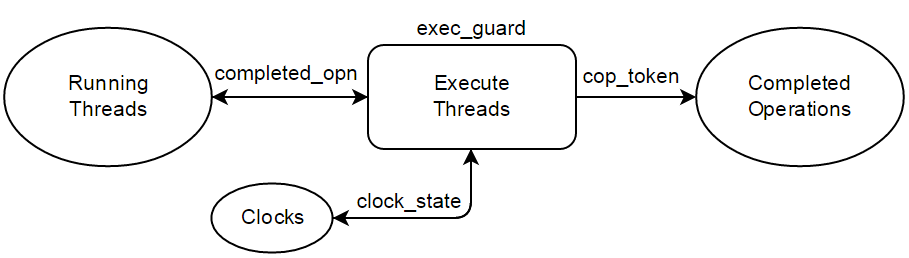
\includegraphics[width=0.48\textwidth]{figs/Response_Times.png}
	\caption{Response-time Analysis}
	\label{fig:COP}
\end{figure}

\subsubsection{Response-time Analysis}

Response-times are measured by observing completed operations. Similar to deadline violations, an observer place \emph{Completed Operations} (Figure \ref{fig:COP}) accumulates all operation requests completed by component threads on all nodes. The structure of this data is similar to equation \ref{eq:DLV} except we replace $O_{DLT}$ with the end-time of the operation $O_{ET}$.

For a known trigger operation and an expected response/actuation, we used state space queries to identify the (1) earliest completion of the trigger operation and the (2) latest completion of a response operation. These operations are possibly running on different components, temporal partitions or nodes. To keep a check on the state space for large models, we simply observe the bindings of the transition \emph{Execute Thread} to gather a list of completed operations, ordered by $O_{ET}$.

\subsubsection{Search Results}

Table \ref{table:AR} shows some worst-case execution time results from state space analysis on each component thread on Satellite 1. Each operation request is enqueued into the component message queue at $T_{NQ}$. A dispatcher thread dequeues this request at $T_{DQ}$ and schedules an operation for execution. Delays in the dequeue can be caused due to the non-preemptive nature of the component-level scheduling. Once scheduled, the component executor thread sequentially executes the steps in each operation to completion at time stamp $T_{FIN}$ leading to an overall execution time of $T_{EXEC}$ measured starting from $T_{NQ}$. 

Significant worst-case network delays are assumed between interacting components that are distributed. For instance, the GPS component on each node finishes publishing sensor data at time stamp 8 ms but the GPS components on other nodes do not notice the subscription token in the message queues till $T_{NQ} = 20 ms$. Also, the synchronous dependency of the Flight Control component with the GPS component is a sign of poor design as a scatter command received in partition 2 of one hyperperiod will most likely finish only a hyperperiod later as the updated GPS coordinates are queried. 

\subsubsection{Incomplete Designs}

In order to integrate this analysis approach into early stages of component-based design, we have looked into scenarios where this work is appropriate. As mentioned in Section \ref{subsec:Operation_Deadlines}, a component thread derives its deadlines from the operations it executes. These operations are triggered by requests from external entities with varying priorities. Identifying the optimal priority-assignment scheme for a set of component threads is non-trivial due to these variations. However, initial designs are often specified by timing requirements between system entities. Therefore, for scenarios where the developers are aware of minimum timing requirements but not thread execution orders or OS-level priorities, we have applied this approach to identify partial thread execution orders to refine incomplete designs. 

Consider a sample application that consists of 6 components servicing operation requests. Components threads 1, 2, and 3 are assigned to Partition 1 and threads 4, 5, and 6 are assigned to Partition 2. The thread priorities and execution orders are unknown. Each component is triggered by a timer once every major frame, taking up to 8 ms to complete the callback operation. Assuming a designer requires that operation 3 (handled by thread 3) must complete before 20 ms and operation 5 (handled by thread 5) must complete before 60 ms from the start of the schedule, the analysis will provide a partial thread execution order that satisfies these requirements. To facilitate this, we assign all the relevant threads equal priorities. If all the triggering timers expire at the beginning of the partition schedule, then all component threads become eligible for execution and the OS scheduler uses a non-deterministic round-robin scheduling scheme. By querying the bounded state space that encapsulates this behavior, we arrive at a partial thread scheduling order that satisfies our requirements e.g. thread 3 is scheduled first in partition 1 and thread 5 is scheduled first in partition 2.

\subsection{Discussion}

\subsubsection{Conservative Results}

Using estimates of worst-case execution time for component operations is motivated by the need to make exaggerated assumptions about the system behavior. Pessimistic estimates are a necessary requirement when verifying safety-critical DRE systems. Schedulability analysis with such assumptions should strictly provide conservative results. This means that:

\begin{itemize}
	\item If the analysis results show the possibility of a deadline violation but the deployed system does not, the obtained result is a conservative one as it assumes worst-case behavior. 
	
	\item If the analysis results do not show any timing violations but the deployed system violates response time requirements, deadlines etc., then the analysis does not provide a conservative result and has failed to verify system behavior.
\end{itemize}

In order to guarantee conservative results, the analysis must include worst-case behaviors of all system-level threads that run at higher priority than component threads and are not necessarily modeled by the design-time tools. These threads can be grouped into a set of critical processes with approximations made to simulate the behavior of system-level threads such as (1) globally periodic CPU utilization, (2) CPU utilization for some WCET per partition etc. The best approximation is chosen based on the expected behavior of such critical processes. Best-effort processes are ignored as they always run at a priority lower than the lowest-priority component thread.


\subsubsection{Scalability}
One of the main concerns in comprehensive design-time analysis of this kind is scalability. As the determinism in the initial design increases, the number of possible behaviors and therefore the size of the state space decreases. In essence, the effort required for the analysis to be useful to the designer is dependent heavily on the initial design itself. Increasing the number of equally prioritized components will exponentially increase the number of state space nodes required to accumulate the set of behaviors that are exhibited by the components. In \cite{MoDeVVa}, we presented results showing our analysis model scaling well for medium-sized applications tested up to a 100 mixed-criticality components distributed on up to 5 computing nodes. Although these results were based on design models that made some unrealistic assumptions e.g. 100 timers expiring at the same time and triggering interactions, we have used some heuristics to reduce the generated state space and improve the performance of the search methods. 
\paragraph{Symmetry}
One of the main advantages of using component-based design for complex systems is reusability. It is not unusual to deploy instances of the same application with the same component assembly on multiple computing nodes. If these applications are deployed on symmetrical nodes, the observed state space of behaviors are also symmetrical. To enable efficient search through symmetrical state spaces, we use symmetry-based state space reduction techniques \cite{Kristensen2000} to improve the performance. In Figure \ref{fig:hl_cpn}, to model 100 timers, we moved from using 100 colored tokens in the \emph{Timers} place to using a single token which is a list consisting of a 100 elements. This way, when multiple timers expire, a single transition firing handles all the expiries across all nodes (a single state change) instead of multiple transition firings leading to multiple new states. This works well when a single instance of an application is deployed on several computing nodes with little non-determinism. The non-determinism caused by the OS-level scheduling of components and component-level operation request collisions still cause the state space to grow across symmetric nodes. 
\paragraph{ASAP Tool}
The CPN Tools GUI contributes to inefficient performance of state space generation for large CPN models. This is significantly improved by using the ASAP \cite{ASAP} analysis tool. The tool provides for several search algorithms and state space reduction techniques such as the \emph{sweep-line method} \cite{Christensen2001} which deletes already visited state space nodes from memory, forcing on-the-fly verification of temporal properties. One of the disadvantages of using such heuristics is the run-time cost incurred by backward-generation of states when a backtrace for a violation is required. However, if a path from the initial state to an inconsistent state is not desired, a combination of this method and the symmetry method reduces the state space and improves verification performance.  


\section{Integration of Modeling Tools}
\label{sec:IMT}

This section briefly describes the integration of the CPN-based analysis with the design-time modeling tools for automated model transformations and generation. For large applications with multiple computing nodes, application instances and component assemblies, hand-writing the CPN token specifications will prove to be cumbersome and error prone. This is avoided completely by parsing the domain-specific model of the system, obtaining necessary structural and behavioral attributes and using a model interpreter to generate a valid CPN model for the design.

\subsection{Timing Specification for Component Operations}

As mentioned in Section \ref{para:steps}, every component operation is modeled as a sequence of functional steps, each with an assigned worst-case execution time. When scheduled, these operations execute one step at a time. Our goal with this specification is to be able to model these sequential steps. We broadly classified these steps into (1) local uninvolved code blocks, (2) peer-to-peer synchronous and asynchronous remote calls, (3) anonymous publish/subscribe distribution services, (4) blocking  and non-blocking I/O interactions and (5) control loops. The restriction to these 5 types is a consequence of the coupling with the DREMS component model and can be easily expanded. 

\begin{figure}[htb]
	\centering
	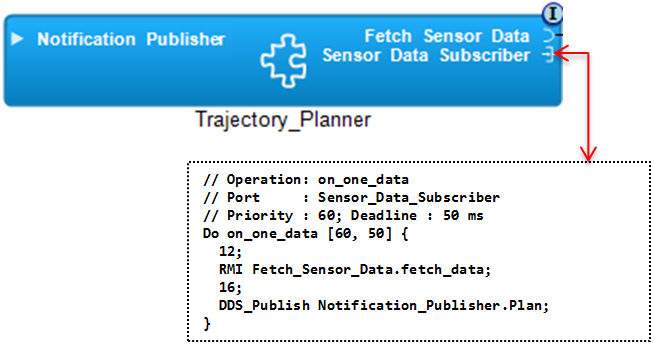
\includegraphics[width=0.40\textwidth]{figs/Timing_Specification.png}
	\caption{Timing Specification for Component Operation}
	\label{fig:ANTLR}
\end{figure}

Figure \ref{fig:ANTLR} shows the %ANTLR-based 
temporal specification for the operation \emph{on\_one\_data} residing in Component \emph{Trajectory\_Planner} exposed through the \emph{Sensor\_Data\_Subscriber} port. This port subscribes to sensor data published by another component using \emph{Push Subscription} semantics. On reception of sensor data, the operation on\_one\_data is called, triggering a sequence of events. Abstracting the business logic, this operation has 4 execution steps: (1) Local \emph{work} for  12 ms, followed by an (3) RMI call to the remote method \emph{fetch\_data} using the \emph{Fetch\_Sensor\_Data} receptacle port, (3) 16 ms of local work, and finally (4) publishing a \emph{Plan} data structure anonymously using the \emph{Notification\_Publisher} port.   

\subsection{Model Generation}

CPN Tools saves colored Petri nets using an XML-based text template. The goal of model generation is to accurately generate a valid \emph{.cpn} file from the domain-specific model of the component-based application. A model interpreter parses the design model diagrams and accumulates data structures representing the various CPN tokens described in Section \ref{sec:Colored_Petri Net-based_Analysis_Model}. This includes structural properties like component assembly and software deployment, temporal properties like scheduling schemes, operation execution times and instanced deployment where a single application can be deployed simultaneously on multiple computing nodes. Figure \ref{fig:GT} shows the token structure generated for the on\_one\_data operation.

\begin{figure}[htb]
	\centering
	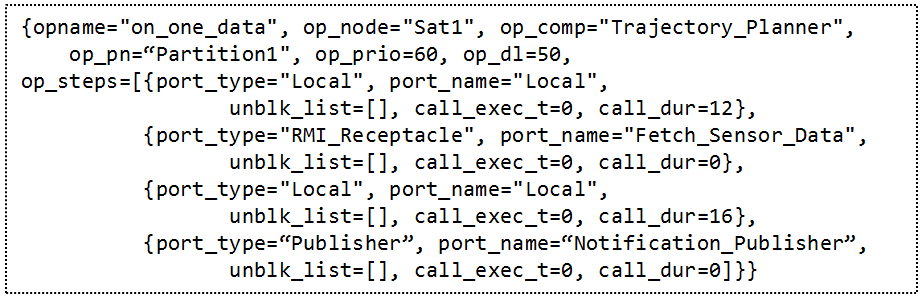
\includegraphics[width=0.48\textwidth]{figs/Generated_Token.png}
	\caption{on\_one\_data CPN token}
	\label{fig:GT}
\end{figure}

Using run-time text templates \cite{T4TextTemplates}, a modular and hierarchical CPN model is generated. This CPN model is accompanied by a set of \emph{.sml} function files that dictate the behavior of the CPN transitions, guards and arc bindings. Using parameters in the design model, these functions can be easily interchanged to tweak the behavior of the analysis model e.g. component-level EDF or FIFO scheduling, OS-level scheduling schemes and state space analysis options.


